
\begin{figure}[h]
\centering
\resizebox{\textwidth}{!}{
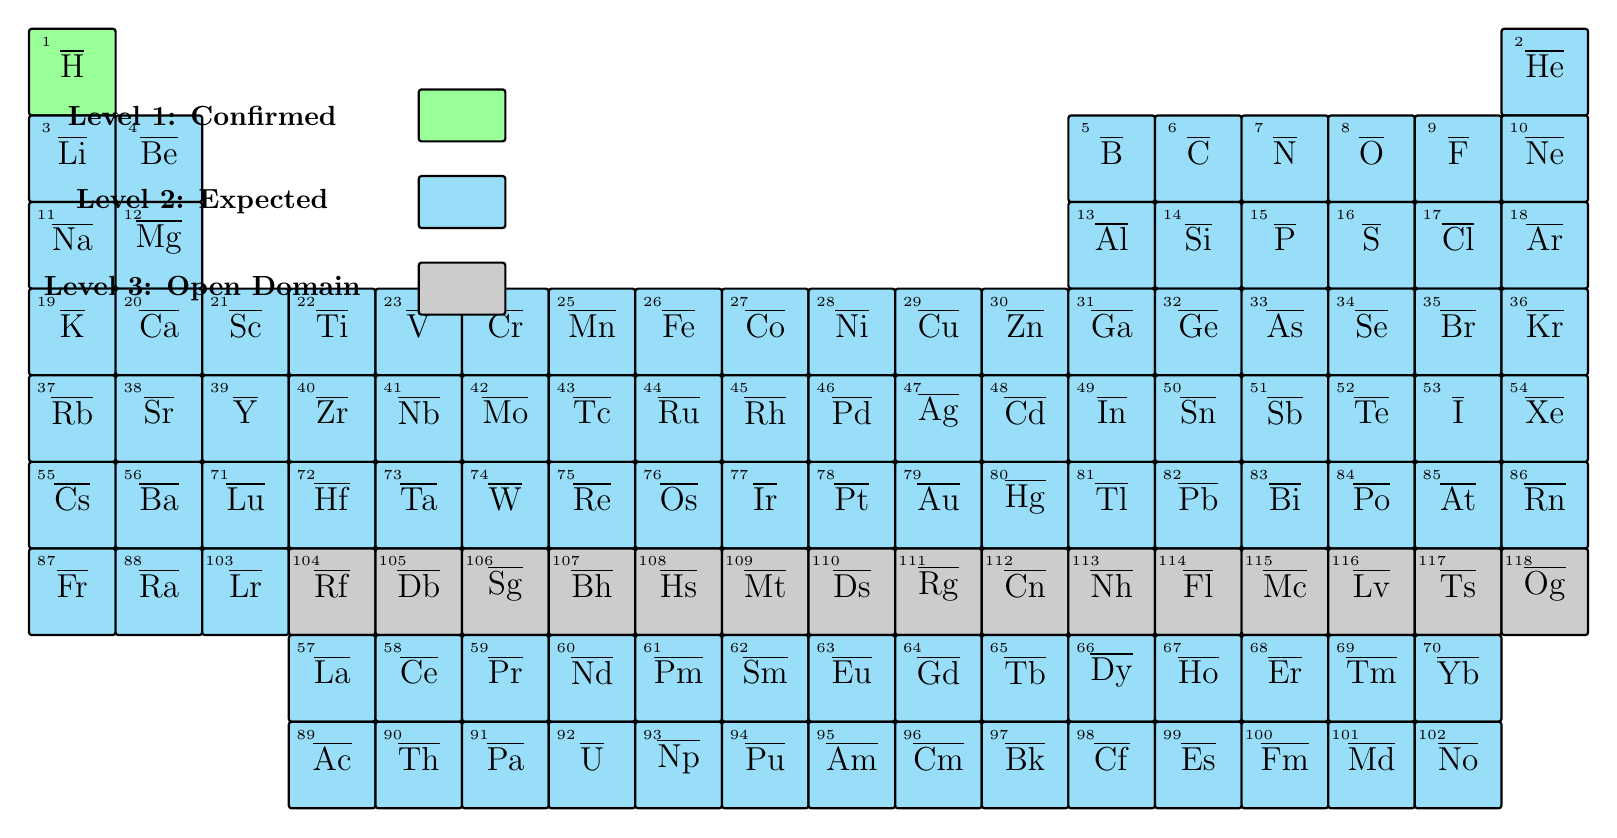
\begin{tikzpicture}[x=1.1cm, y=1.1cm]
\draw[fill=green!40, draw=black, thick, rounded corners=1pt] (0,0) rectangle (1,-1);
\node at (0.5,-0.4) {\large \textbf{$\overline{\mathrm{H}}$}};
\node at (0.2,-0.15) {\tiny 1};
\draw[fill=cyan!40, draw=black, thick, rounded corners=1pt] (17,0) rectangle (18,-1);
\node at (17.5,-0.4) {\large \textbf{$\overline{\mathrm{He}}$}};
\node at (17.2,-0.15) {\tiny 2};
\draw[fill=cyan!40, draw=black, thick, rounded corners=1pt] (0,-1) rectangle (1,-2);
\node at (0.5,-1.4) {\large \textbf{$\overline{\mathrm{Li}}$}};
\node at (0.2,-1.15) {\tiny 3};
\draw[fill=cyan!40, draw=black, thick, rounded corners=1pt] (1,-1) rectangle (2,-2);
\node at (1.5,-1.4) {\large \textbf{$\overline{\mathrm{Be}}$}};
\node at (1.2,-1.15) {\tiny 4};
\draw[fill=cyan!40, draw=black, thick, rounded corners=1pt] (12,-1) rectangle (13,-2);
\node at (12.5,-1.4) {\large \textbf{$\overline{\mathrm{B}}$}};
\node at (12.2,-1.15) {\tiny 5};
\draw[fill=cyan!40, draw=black, thick, rounded corners=1pt] (13,-1) rectangle (14,-2);
\node at (13.5,-1.4) {\large \textbf{$\overline{\mathrm{C}}$}};
\node at (13.2,-1.15) {\tiny 6};
\draw[fill=cyan!40, draw=black, thick, rounded corners=1pt] (14,-1) rectangle (15,-2);
\node at (14.5,-1.4) {\large \textbf{$\overline{\mathrm{N}}$}};
\node at (14.2,-1.15) {\tiny 7};
\draw[fill=cyan!40, draw=black, thick, rounded corners=1pt] (15,-1) rectangle (16,-2);
\node at (15.5,-1.4) {\large \textbf{$\overline{\mathrm{O}}$}};
\node at (15.2,-1.15) {\tiny 8};
\draw[fill=cyan!40, draw=black, thick, rounded corners=1pt] (16,-1) rectangle (17,-2);
\node at (16.5,-1.4) {\large \textbf{$\overline{\mathrm{F}}$}};
\node at (16.2,-1.15) {\tiny 9};
\draw[fill=cyan!40, draw=black, thick, rounded corners=1pt] (17,-1) rectangle (18,-2);
\node at (17.5,-1.4) {\large \textbf{$\overline{\mathrm{Ne}}$}};
\node at (17.2,-1.15) {\tiny 10};
\draw[fill=cyan!40, draw=black, thick, rounded corners=1pt] (0,-2) rectangle (1,-3);
\node at (0.5,-2.4) {\large \textbf{$\overline{\mathrm{Na}}$}};
\node at (0.2,-2.15) {\tiny 11};
\draw[fill=cyan!40, draw=black, thick, rounded corners=1pt] (1,-2) rectangle (2,-3);
\node at (1.5,-2.4) {\large \textbf{$\overline{\mathrm{Mg}}$}};
\node at (1.2,-2.15) {\tiny 12};
\draw[fill=cyan!40, draw=black, thick, rounded corners=1pt] (12,-2) rectangle (13,-3);
\node at (12.5,-2.4) {\large \textbf{$\overline{\mathrm{Al}}$}};
\node at (12.2,-2.15) {\tiny 13};
\draw[fill=cyan!40, draw=black, thick, rounded corners=1pt] (13,-2) rectangle (14,-3);
\node at (13.5,-2.4) {\large \textbf{$\overline{\mathrm{Si}}$}};
\node at (13.2,-2.15) {\tiny 14};
\draw[fill=cyan!40, draw=black, thick, rounded corners=1pt] (14,-2) rectangle (15,-3);
\node at (14.5,-2.4) {\large \textbf{$\overline{\mathrm{P}}$}};
\node at (14.2,-2.15) {\tiny 15};
\draw[fill=cyan!40, draw=black, thick, rounded corners=1pt] (15,-2) rectangle (16,-3);
\node at (15.5,-2.4) {\large \textbf{$\overline{\mathrm{S}}$}};
\node at (15.2,-2.15) {\tiny 16};
\draw[fill=cyan!40, draw=black, thick, rounded corners=1pt] (16,-2) rectangle (17,-3);
\node at (16.5,-2.4) {\large \textbf{$\overline{\mathrm{Cl}}$}};
\node at (16.2,-2.15) {\tiny 17};
\draw[fill=cyan!40, draw=black, thick, rounded corners=1pt] (17,-2) rectangle (18,-3);
\node at (17.5,-2.4) {\large \textbf{$\overline{\mathrm{Ar}}$}};
\node at (17.2,-2.15) {\tiny 18};
\draw[fill=cyan!40, draw=black, thick, rounded corners=1pt] (0,-3) rectangle (1,-4);
\node at (0.5,-3.4) {\large \textbf{$\overline{\mathrm{K}}$}};
\node at (0.2,-3.15) {\tiny 19};
\draw[fill=cyan!40, draw=black, thick, rounded corners=1pt] (1,-3) rectangle (2,-4);
\node at (1.5,-3.4) {\large \textbf{$\overline{\mathrm{Ca}}$}};
\node at (1.2,-3.15) {\tiny 20};
\draw[fill=cyan!40, draw=black, thick, rounded corners=1pt] (2,-3) rectangle (3,-4);
\node at (2.5,-3.4) {\large \textbf{$\overline{\mathrm{Sc}}$}};
\node at (2.2,-3.15) {\tiny 21};
\draw[fill=cyan!40, draw=black, thick, rounded corners=1pt] (3,-3) rectangle (4,-4);
\node at (3.5,-3.4) {\large \textbf{$\overline{\mathrm{Ti}}$}};
\node at (3.2,-3.15) {\tiny 22};
\draw[fill=cyan!40, draw=black, thick, rounded corners=1pt] (4,-3) rectangle (5,-4);
\node at (4.5,-3.4) {\large \textbf{$\overline{\mathrm{V}}$}};
\node at (4.2,-3.15) {\tiny 23};
\draw[fill=cyan!40, draw=black, thick, rounded corners=1pt] (5,-3) rectangle (6,-4);
\node at (5.5,-3.4) {\large \textbf{$\overline{\mathrm{Cr}}$}};
\node at (5.2,-3.15) {\tiny 24};
\draw[fill=cyan!40, draw=black, thick, rounded corners=1pt] (6,-3) rectangle (7,-4);
\node at (6.5,-3.4) {\large \textbf{$\overline{\mathrm{Mn}}$}};
\node at (6.2,-3.15) {\tiny 25};
\draw[fill=cyan!40, draw=black, thick, rounded corners=1pt] (7,-3) rectangle (8,-4);
\node at (7.5,-3.4) {\large \textbf{$\overline{\mathrm{Fe}}$}};
\node at (7.2,-3.15) {\tiny 26};
\draw[fill=cyan!40, draw=black, thick, rounded corners=1pt] (8,-3) rectangle (9,-4);
\node at (8.5,-3.4) {\large \textbf{$\overline{\mathrm{Co}}$}};
\node at (8.2,-3.15) {\tiny 27};
\draw[fill=cyan!40, draw=black, thick, rounded corners=1pt] (9,-3) rectangle (10,-4);
\node at (9.5,-3.4) {\large \textbf{$\overline{\mathrm{Ni}}$}};
\node at (9.2,-3.15) {\tiny 28};
\draw[fill=cyan!40, draw=black, thick, rounded corners=1pt] (10,-3) rectangle (11,-4);
\node at (10.5,-3.4) {\large \textbf{$\overline{\mathrm{Cu}}$}};
\node at (10.2,-3.15) {\tiny 29};
\draw[fill=cyan!40, draw=black, thick, rounded corners=1pt] (11,-3) rectangle (12,-4);
\node at (11.5,-3.4) {\large \textbf{$\overline{\mathrm{Zn}}$}};
\node at (11.2,-3.15) {\tiny 30};
\draw[fill=cyan!40, draw=black, thick, rounded corners=1pt] (12,-3) rectangle (13,-4);
\node at (12.5,-3.4) {\large \textbf{$\overline{\mathrm{Ga}}$}};
\node at (12.2,-3.15) {\tiny 31};
\draw[fill=cyan!40, draw=black, thick, rounded corners=1pt] (13,-3) rectangle (14,-4);
\node at (13.5,-3.4) {\large \textbf{$\overline{\mathrm{Ge}}$}};
\node at (13.2,-3.15) {\tiny 32};
\draw[fill=cyan!40, draw=black, thick, rounded corners=1pt] (14,-3) rectangle (15,-4);
\node at (14.5,-3.4) {\large \textbf{$\overline{\mathrm{As}}$}};
\node at (14.2,-3.15) {\tiny 33};
\draw[fill=cyan!40, draw=black, thick, rounded corners=1pt] (15,-3) rectangle (16,-4);
\node at (15.5,-3.4) {\large \textbf{$\overline{\mathrm{Se}}$}};
\node at (15.2,-3.15) {\tiny 34};
\draw[fill=cyan!40, draw=black, thick, rounded corners=1pt] (16,-3) rectangle (17,-4);
\node at (16.5,-3.4) {\large \textbf{$\overline{\mathrm{Br}}$}};
\node at (16.2,-3.15) {\tiny 35};
\draw[fill=cyan!40, draw=black, thick, rounded corners=1pt] (17,-3) rectangle (18,-4);
\node at (17.5,-3.4) {\large \textbf{$\overline{\mathrm{Kr}}$}};
\node at (17.2,-3.15) {\tiny 36};
\draw[fill=cyan!40, draw=black, thick, rounded corners=1pt] (0,-4) rectangle (1,-5);
\node at (0.5,-4.4) {\large \textbf{$\overline{\mathrm{Rb}}$}};
\node at (0.2,-4.15) {\tiny 37};
\draw[fill=cyan!40, draw=black, thick, rounded corners=1pt] (1,-4) rectangle (2,-5);
\node at (1.5,-4.4) {\large \textbf{$\overline{\mathrm{Sr}}$}};
\node at (1.2,-4.15) {\tiny 38};
\draw[fill=cyan!40, draw=black, thick, rounded corners=1pt] (2,-4) rectangle (3,-5);
\node at (2.5,-4.4) {\large \textbf{$\overline{\mathrm{Y}}$}};
\node at (2.2,-4.15) {\tiny 39};
\draw[fill=cyan!40, draw=black, thick, rounded corners=1pt] (3,-4) rectangle (4,-5);
\node at (3.5,-4.4) {\large \textbf{$\overline{\mathrm{Zr}}$}};
\node at (3.2,-4.15) {\tiny 40};
\draw[fill=cyan!40, draw=black, thick, rounded corners=1pt] (4,-4) rectangle (5,-5);
\node at (4.5,-4.4) {\large \textbf{$\overline{\mathrm{Nb}}$}};
\node at (4.2,-4.15) {\tiny 41};
\draw[fill=cyan!40, draw=black, thick, rounded corners=1pt] (5,-4) rectangle (6,-5);
\node at (5.5,-4.4) {\large \textbf{$\overline{\mathrm{Mo}}$}};
\node at (5.2,-4.15) {\tiny 42};
\draw[fill=cyan!40, draw=black, thick, rounded corners=1pt] (6,-4) rectangle (7,-5);
\node at (6.5,-4.4) {\large \textbf{$\overline{\mathrm{Tc}}$}};
\node at (6.2,-4.15) {\tiny 43};
\draw[fill=cyan!40, draw=black, thick, rounded corners=1pt] (7,-4) rectangle (8,-5);
\node at (7.5,-4.4) {\large \textbf{$\overline{\mathrm{Ru}}$}};
\node at (7.2,-4.15) {\tiny 44};
\draw[fill=cyan!40, draw=black, thick, rounded corners=1pt] (8,-4) rectangle (9,-5);
\node at (8.5,-4.4) {\large \textbf{$\overline{\mathrm{Rh}}$}};
\node at (8.2,-4.15) {\tiny 45};
\draw[fill=cyan!40, draw=black, thick, rounded corners=1pt] (9,-4) rectangle (10,-5);
\node at (9.5,-4.4) {\large \textbf{$\overline{\mathrm{Pd}}$}};
\node at (9.2,-4.15) {\tiny 46};
\draw[fill=cyan!40, draw=black, thick, rounded corners=1pt] (10,-4) rectangle (11,-5);
\node at (10.5,-4.4) {\large \textbf{$\overline{\mathrm{Ag}}$}};
\node at (10.2,-4.15) {\tiny 47};
\draw[fill=cyan!40, draw=black, thick, rounded corners=1pt] (11,-4) rectangle (12,-5);
\node at (11.5,-4.4) {\large \textbf{$\overline{\mathrm{Cd}}$}};
\node at (11.2,-4.15) {\tiny 48};
\draw[fill=cyan!40, draw=black, thick, rounded corners=1pt] (12,-4) rectangle (13,-5);
\node at (12.5,-4.4) {\large \textbf{$\overline{\mathrm{In}}$}};
\node at (12.2,-4.15) {\tiny 49};
\draw[fill=cyan!40, draw=black, thick, rounded corners=1pt] (13,-4) rectangle (14,-5);
\node at (13.5,-4.4) {\large \textbf{$\overline{\mathrm{Sn}}$}};
\node at (13.2,-4.15) {\tiny 50};
\draw[fill=cyan!40, draw=black, thick, rounded corners=1pt] (14,-4) rectangle (15,-5);
\node at (14.5,-4.4) {\large \textbf{$\overline{\mathrm{Sb}}$}};
\node at (14.2,-4.15) {\tiny 51};
\draw[fill=cyan!40, draw=black, thick, rounded corners=1pt] (15,-4) rectangle (16,-5);
\node at (15.5,-4.4) {\large \textbf{$\overline{\mathrm{Te}}$}};
\node at (15.2,-4.15) {\tiny 52};
\draw[fill=cyan!40, draw=black, thick, rounded corners=1pt] (16,-4) rectangle (17,-5);
\node at (16.5,-4.4) {\large \textbf{$\overline{\mathrm{I}}$}};
\node at (16.2,-4.15) {\tiny 53};
\draw[fill=cyan!40, draw=black, thick, rounded corners=1pt] (17,-4) rectangle (18,-5);
\node at (17.5,-4.4) {\large \textbf{$\overline{\mathrm{Xe}}$}};
\node at (17.2,-4.15) {\tiny 54};
\draw[fill=cyan!40, draw=black, thick, rounded corners=1pt] (0,-5) rectangle (1,-6);
\node at (0.5,-5.4) {\large \textbf{$\overline{\mathrm{Cs}}$}};
\node at (0.2,-5.15) {\tiny 55};
\draw[fill=cyan!40, draw=black, thick, rounded corners=1pt] (1,-5) rectangle (2,-6);
\node at (1.5,-5.4) {\large \textbf{$\overline{\mathrm{Ba}}$}};
\node at (1.2,-5.15) {\tiny 56};
\draw[fill=cyan!40, draw=black, thick, rounded corners=1pt] (2,-5) rectangle (3,-6);
\node at (2.5,-5.4) {\large \textbf{$\overline{\mathrm{Lu}}$}};
\node at (2.2,-5.15) {\tiny 71};
\draw[fill=cyan!40, draw=black, thick, rounded corners=1pt] (3,-5) rectangle (4,-6);
\node at (3.5,-5.4) {\large \textbf{$\overline{\mathrm{Hf}}$}};
\node at (3.2,-5.15) {\tiny 72};
\draw[fill=cyan!40, draw=black, thick, rounded corners=1pt] (4,-5) rectangle (5,-6);
\node at (4.5,-5.4) {\large \textbf{$\overline{\mathrm{Ta}}$}};
\node at (4.2,-5.15) {\tiny 73};
\draw[fill=cyan!40, draw=black, thick, rounded corners=1pt] (5,-5) rectangle (6,-6);
\node at (5.5,-5.4) {\large \textbf{$\overline{\mathrm{W}}$}};
\node at (5.2,-5.15) {\tiny 74};
\draw[fill=cyan!40, draw=black, thick, rounded corners=1pt] (6,-5) rectangle (7,-6);
\node at (6.5,-5.4) {\large \textbf{$\overline{\mathrm{Re}}$}};
\node at (6.2,-5.15) {\tiny 75};
\draw[fill=cyan!40, draw=black, thick, rounded corners=1pt] (7,-5) rectangle (8,-6);
\node at (7.5,-5.4) {\large \textbf{$\overline{\mathrm{Os}}$}};
\node at (7.2,-5.15) {\tiny 76};
\draw[fill=cyan!40, draw=black, thick, rounded corners=1pt] (8,-5) rectangle (9,-6);
\node at (8.5,-5.4) {\large \textbf{$\overline{\mathrm{Ir}}$}};
\node at (8.2,-5.15) {\tiny 77};
\draw[fill=cyan!40, draw=black, thick, rounded corners=1pt] (9,-5) rectangle (10,-6);
\node at (9.5,-5.4) {\large \textbf{$\overline{\mathrm{Pt}}$}};
\node at (9.2,-5.15) {\tiny 78};
\draw[fill=cyan!40, draw=black, thick, rounded corners=1pt] (10,-5) rectangle (11,-6);
\node at (10.5,-5.4) {\large \textbf{$\overline{\mathrm{Au}}$}};
\node at (10.2,-5.15) {\tiny 79};
\draw[fill=cyan!40, draw=black, thick, rounded corners=1pt] (11,-5) rectangle (12,-6);
\node at (11.5,-5.4) {\large \textbf{$\overline{\mathrm{Hg}}$}};
\node at (11.2,-5.15) {\tiny 80};
\draw[fill=cyan!40, draw=black, thick, rounded corners=1pt] (12,-5) rectangle (13,-6);
\node at (12.5,-5.4) {\large \textbf{$\overline{\mathrm{Tl}}$}};
\node at (12.2,-5.15) {\tiny 81};
\draw[fill=cyan!40, draw=black, thick, rounded corners=1pt] (13,-5) rectangle (14,-6);
\node at (13.5,-5.4) {\large \textbf{$\overline{\mathrm{Pb}}$}};
\node at (13.2,-5.15) {\tiny 82};
\draw[fill=cyan!40, draw=black, thick, rounded corners=1pt] (14,-5) rectangle (15,-6);
\node at (14.5,-5.4) {\large \textbf{$\overline{\mathrm{Bi}}$}};
\node at (14.2,-5.15) {\tiny 83};
\draw[fill=cyan!40, draw=black, thick, rounded corners=1pt] (15,-5) rectangle (16,-6);
\node at (15.5,-5.4) {\large \textbf{$\overline{\mathrm{Po}}$}};
\node at (15.2,-5.15) {\tiny 84};
\draw[fill=cyan!40, draw=black, thick, rounded corners=1pt] (16,-5) rectangle (17,-6);
\node at (16.5,-5.4) {\large \textbf{$\overline{\mathrm{At}}$}};
\node at (16.2,-5.15) {\tiny 85};
\draw[fill=cyan!40, draw=black, thick, rounded corners=1pt] (17,-5) rectangle (18,-6);
\node at (17.5,-5.4) {\large \textbf{$\overline{\mathrm{Rn}}$}};
\node at (17.2,-5.15) {\tiny 86};
\draw[fill=cyan!40, draw=black, thick, rounded corners=1pt] (0,-6) rectangle (1,-7);
\node at (0.5,-6.4) {\large \textbf{$\overline{\mathrm{Fr}}$}};
\node at (0.2,-6.15) {\tiny 87};
\draw[fill=cyan!40, draw=black, thick, rounded corners=1pt] (1,-6) rectangle (2,-7);
\node at (1.5,-6.4) {\large \textbf{$\overline{\mathrm{Ra}}$}};
\node at (1.2,-6.15) {\tiny 88};
\draw[fill=cyan!40, draw=black, thick, rounded corners=1pt] (2,-6) rectangle (3,-7);
\node at (2.5,-6.4) {\large \textbf{$\overline{\mathrm{Lr}}$}};
\node at (2.2,-6.15) {\tiny 103};
\draw[fill=gray!40, draw=black, thick, rounded corners=1pt] (3,-6) rectangle (4,-7);
\node at (3.5,-6.4) {\large \textbf{$\overline{\mathrm{Rf}}$}};
\node at (3.2,-6.15) {\tiny 104};
\draw[fill=gray!40, draw=black, thick, rounded corners=1pt] (4,-6) rectangle (5,-7);
\node at (4.5,-6.4) {\large \textbf{$\overline{\mathrm{Db}}$}};
\node at (4.2,-6.15) {\tiny 105};
\draw[fill=gray!40, draw=black, thick, rounded corners=1pt] (5,-6) rectangle (6,-7);
\node at (5.5,-6.4) {\large \textbf{$\overline{\mathrm{Sg}}$}};
\node at (5.2,-6.15) {\tiny 106};
\draw[fill=gray!40, draw=black, thick, rounded corners=1pt] (6,-6) rectangle (7,-7);
\node at (6.5,-6.4) {\large \textbf{$\overline{\mathrm{Bh}}$}};
\node at (6.2,-6.15) {\tiny 107};
\draw[fill=gray!40, draw=black, thick, rounded corners=1pt] (7,-6) rectangle (8,-7);
\node at (7.5,-6.4) {\large \textbf{$\overline{\mathrm{Hs}}$}};
\node at (7.2,-6.15) {\tiny 108};
\draw[fill=gray!40, draw=black, thick, rounded corners=1pt] (8,-6) rectangle (9,-7);
\node at (8.5,-6.4) {\large \textbf{$\overline{\mathrm{Mt}}$}};
\node at (8.2,-6.15) {\tiny 109};
\draw[fill=gray!40, draw=black, thick, rounded corners=1pt] (9,-6) rectangle (10,-7);
\node at (9.5,-6.4) {\large \textbf{$\overline{\mathrm{Ds}}$}};
\node at (9.2,-6.15) {\tiny 110};
\draw[fill=gray!40, draw=black, thick, rounded corners=1pt] (10,-6) rectangle (11,-7);
\node at (10.5,-6.4) {\large \textbf{$\overline{\mathrm{Rg}}$}};
\node at (10.2,-6.15) {\tiny 111};
\draw[fill=gray!40, draw=black, thick, rounded corners=1pt] (11,-6) rectangle (12,-7);
\node at (11.5,-6.4) {\large \textbf{$\overline{\mathrm{Cn}}$}};
\node at (11.2,-6.15) {\tiny 112};
\draw[fill=gray!40, draw=black, thick, rounded corners=1pt] (12,-6) rectangle (13,-7);
\node at (12.5,-6.4) {\large \textbf{$\overline{\mathrm{Nh}}$}};
\node at (12.2,-6.15) {\tiny 113};
\draw[fill=gray!40, draw=black, thick, rounded corners=1pt] (13,-6) rectangle (14,-7);
\node at (13.5,-6.4) {\large \textbf{$\overline{\mathrm{Fl}}$}};
\node at (13.2,-6.15) {\tiny 114};
\draw[fill=gray!40, draw=black, thick, rounded corners=1pt] (14,-6) rectangle (15,-7);
\node at (14.5,-6.4) {\large \textbf{$\overline{\mathrm{Mc}}$}};
\node at (14.2,-6.15) {\tiny 115};
\draw[fill=gray!40, draw=black, thick, rounded corners=1pt] (15,-6) rectangle (16,-7);
\node at (15.5,-6.4) {\large \textbf{$\overline{\mathrm{Lv}}$}};
\node at (15.2,-6.15) {\tiny 116};
\draw[fill=gray!40, draw=black, thick, rounded corners=1pt] (16,-6) rectangle (17,-7);
\node at (16.5,-6.4) {\large \textbf{$\overline{\mathrm{Ts}}$}};
\node at (16.2,-6.15) {\tiny 117};
\draw[fill=gray!40, draw=black, thick, rounded corners=1pt] (17,-6) rectangle (18,-7);
\node at (17.5,-6.4) {\large \textbf{$\overline{\mathrm{Og}}$}};
\node at (17.2,-6.15) {\tiny 118};
\draw[fill=cyan!40, draw=black, thick, rounded corners=1pt] (3,-7) rectangle (4,-8);
\node at (3.5,-7.4) {\large \textbf{$\overline{\mathrm{La}}$}};
\node at (3.2,-7.15) {\tiny 57};
\draw[fill=cyan!40, draw=black, thick, rounded corners=1pt] (4,-7) rectangle (5,-8);
\node at (4.5,-7.4) {\large \textbf{$\overline{\mathrm{Ce}}$}};
\node at (4.2,-7.15) {\tiny 58};
\draw[fill=cyan!40, draw=black, thick, rounded corners=1pt] (5,-7) rectangle (6,-8);
\node at (5.5,-7.4) {\large \textbf{$\overline{\mathrm{Pr}}$}};
\node at (5.2,-7.15) {\tiny 59};
\draw[fill=cyan!40, draw=black, thick, rounded corners=1pt] (6,-7) rectangle (7,-8);
\node at (6.5,-7.4) {\large \textbf{$\overline{\mathrm{Nd}}$}};
\node at (6.2,-7.15) {\tiny 60};
\draw[fill=cyan!40, draw=black, thick, rounded corners=1pt] (7,-7) rectangle (8,-8);
\node at (7.5,-7.4) {\large \textbf{$\overline{\mathrm{Pm}}$}};
\node at (7.2,-7.15) {\tiny 61};
\draw[fill=cyan!40, draw=black, thick, rounded corners=1pt] (8,-7) rectangle (9,-8);
\node at (8.5,-7.4) {\large \textbf{$\overline{\mathrm{Sm}}$}};
\node at (8.2,-7.15) {\tiny 62};
\draw[fill=cyan!40, draw=black, thick, rounded corners=1pt] (9,-7) rectangle (10,-8);
\node at (9.5,-7.4) {\large \textbf{$\overline{\mathrm{Eu}}$}};
\node at (9.2,-7.15) {\tiny 63};
\draw[fill=cyan!40, draw=black, thick, rounded corners=1pt] (10,-7) rectangle (11,-8);
\node at (10.5,-7.4) {\large \textbf{$\overline{\mathrm{Gd}}$}};
\node at (10.2,-7.15) {\tiny 64};
\draw[fill=cyan!40, draw=black, thick, rounded corners=1pt] (11,-7) rectangle (12,-8);
\node at (11.5,-7.4) {\large \textbf{$\overline{\mathrm{Tb}}$}};
\node at (11.2,-7.15) {\tiny 65};
\draw[fill=cyan!40, draw=black, thick, rounded corners=1pt] (12,-7) rectangle (13,-8);
\node at (12.5,-7.4) {\large \textbf{$\overline{\mathrm{Dy}}$}};
\node at (12.2,-7.15) {\tiny 66};
\draw[fill=cyan!40, draw=black, thick, rounded corners=1pt] (13,-7) rectangle (14,-8);
\node at (13.5,-7.4) {\large \textbf{$\overline{\mathrm{Ho}}$}};
\node at (13.2,-7.15) {\tiny 67};
\draw[fill=cyan!40, draw=black, thick, rounded corners=1pt] (14,-7) rectangle (15,-8);
\node at (14.5,-7.4) {\large \textbf{$\overline{\mathrm{Er}}$}};
\node at (14.2,-7.15) {\tiny 68};
\draw[fill=cyan!40, draw=black, thick, rounded corners=1pt] (15,-7) rectangle (16,-8);
\node at (15.5,-7.4) {\large \textbf{$\overline{\mathrm{Tm}}$}};
\node at (15.2,-7.15) {\tiny 69};
\draw[fill=cyan!40, draw=black, thick, rounded corners=1pt] (16,-7) rectangle (17,-8);
\node at (16.5,-7.4) {\large \textbf{$\overline{\mathrm{Yb}}$}};
\node at (16.2,-7.15) {\tiny 70};
\draw[fill=cyan!40, draw=black, thick, rounded corners=1pt] (3,-8) rectangle (4,-9);
\node at (3.5,-8.4) {\large \textbf{$\overline{\mathrm{Ac}}$}};
\node at (3.2,-8.15) {\tiny 89};
\draw[fill=cyan!40, draw=black, thick, rounded corners=1pt] (4,-8) rectangle (5,-9);
\node at (4.5,-8.4) {\large \textbf{$\overline{\mathrm{Th}}$}};
\node at (4.2,-8.15) {\tiny 90};
\draw[fill=cyan!40, draw=black, thick, rounded corners=1pt] (5,-8) rectangle (6,-9);
\node at (5.5,-8.4) {\large \textbf{$\overline{\mathrm{Pa}}$}};
\node at (5.2,-8.15) {\tiny 91};
\draw[fill=cyan!40, draw=black, thick, rounded corners=1pt] (6,-8) rectangle (7,-9);
\node at (6.5,-8.4) {\large \textbf{$\overline{\mathrm{U}}$}};
\node at (6.2,-8.15) {\tiny 92};
\draw[fill=cyan!40, draw=black, thick, rounded corners=1pt] (7,-8) rectangle (8,-9);
\node at (7.5,-8.4) {\large \textbf{$\overline{\mathrm{Np}}$}};
\node at (7.2,-8.15) {\tiny 93};
\draw[fill=cyan!40, draw=black, thick, rounded corners=1pt] (8,-8) rectangle (9,-9);
\node at (8.5,-8.4) {\large \textbf{$\overline{\mathrm{Pu}}$}};
\node at (8.2,-8.15) {\tiny 94};
\draw[fill=cyan!40, draw=black, thick, rounded corners=1pt] (9,-8) rectangle (10,-9);
\node at (9.5,-8.4) {\large \textbf{$\overline{\mathrm{Am}}$}};
\node at (9.2,-8.15) {\tiny 95};
\draw[fill=cyan!40, draw=black, thick, rounded corners=1pt] (10,-8) rectangle (11,-9);
\node at (10.5,-8.4) {\large \textbf{$\overline{\mathrm{Cm}}$}};
\node at (10.2,-8.15) {\tiny 96};
\draw[fill=cyan!40, draw=black, thick, rounded corners=1pt] (11,-8) rectangle (12,-9);
\node at (11.5,-8.4) {\large \textbf{$\overline{\mathrm{Bk}}$}};
\node at (11.2,-8.15) {\tiny 97};
\draw[fill=cyan!40, draw=black, thick, rounded corners=1pt] (12,-8) rectangle (13,-9);
\node at (12.5,-8.4) {\large \textbf{$\overline{\mathrm{Cf}}$}};
\node at (12.2,-8.15) {\tiny 98};
\draw[fill=cyan!40, draw=black, thick, rounded corners=1pt] (13,-8) rectangle (14,-9);
\node at (13.5,-8.4) {\large \textbf{$\overline{\mathrm{Es}}$}};
\node at (13.2,-8.15) {\tiny 99};
\draw[fill=cyan!40, draw=black, thick, rounded corners=1pt] (14,-8) rectangle (15,-9);
\node at (14.5,-8.4) {\large \textbf{$\overline{\mathrm{Fm}}$}};
\node at (14.2,-8.15) {\tiny 100};
\draw[fill=cyan!40, draw=black, thick, rounded corners=1pt] (15,-8) rectangle (16,-9);
\node at (15.5,-8.4) {\large \textbf{$\overline{\mathrm{Md}}$}};
\node at (15.2,-8.15) {\tiny 101};
\draw[fill=cyan!40, draw=black, thick, rounded corners=1pt] (16,-8) rectangle (17,-9);
\node at (16.5,-8.4) {\large \textbf{$\overline{\mathrm{No}}$}};
\node at (16.2,-8.15) {\tiny 102};

\node at (2, -1) {\textbf{Level 1: Confirmed}};
\draw[fill=green!40, draw=black, thick, rounded corners=1pt] (4.5,-0.7) rectangle (5.5,-1.3);

\node at (2, -2) {\textbf{Level 2: Expected}};
\draw[fill=cyan!40, draw=black, thick, rounded corners=1pt] (4.5,-1.7) rectangle (5.5,-2.3);

\node at (2, -3) {\textbf{Level 3: Open Domain}};
\draw[fill=gray!40, draw=black, thick, rounded corners=1pt] (4.5,-2.7) rectangle (5.5,-3.3);

\end{tikzpicture}
}
\caption{Preparedness Table: Das Antiperiodensystem der Elemente (Statuscodiert)}
\end{figure}
